\chapter{Binary Tree Reduction}
\label{ch:BinaryTreeSummation}

\newcommand{\numLevels}{\lceil \log_2 N \rceil}
\newcommand{\ffs}{\textrm{ffs}}
\newcommand{\nodesum}{\textrm{sum}\,}

\begin{figure}[H]
\centering
\begin{subfigure}{0.45\textwidth}
\centering
\begin{tikzpicture}
% example calculation
\node (A) at (0,-2) {$(3 \reduce 2) \reduce 7$};
\node (B) at (0,-1) {$3 \reduce 2$};
\node (C) at (0,-0) {3};
\node (D) at (1,-0) {2};
\node (E) at (2,-0) {7};
\node (F) at (2,-1) {7};
\draw (C) -- (B);
\draw (B) -- (A);
\draw (D) -- (1,-1) -- (B);
\draw (E) -- (F);
\draw (F) -- (2,-2) -- (A);
\draw (A) -- (0,-3);
\end{tikzpicture}
\caption{Reduction of the elements $3$, $2$, and $7$}
\label{fig:reductionExample}
\end{subfigure}
\hfill
\begin{subfigure}{0.45\textwidth}
\centering
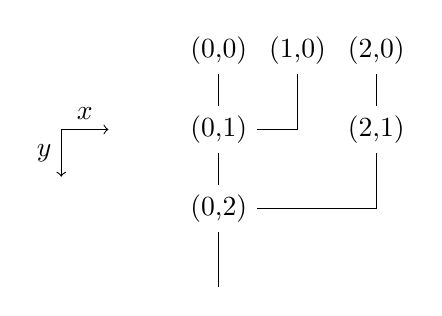
\begin{tikzpicture}
% coordinate system


\coordinate (origin) at (-2,-1);

\draw[->] (origin) -- +(0.6,0) node [above,midway] {$x$};
\draw[->] (origin) -- +(0,-0.6) node [left,midway] {$y$};
\node (A) at (0,-2) {(0,2)};
\node (B) at (0,-1) {(0,1)};
\node (C) at (0,-0) {(0,0)};
\node (D) at (1,-0) {(1,0)};
\node (E) at (2,-0) {(2,0)};
\node (F) at (2,-1) {(2,1)};
\draw (C) -- (B);
\draw (B) -- (A);
\draw (D) -- (1,-1) -- (B);
\draw (E) -- (F);
\draw (F) -- (2,-2) -- (A);
\draw (A) -- (0,-3);
\end{tikzpicture}
\caption{Corresponding coordinate system}
\label{fig:coordinateExample}
\end{subfigure}

\caption{Example reduction tree for $N=3$.}
\label{fig:reductionAndCoordinateExample}
\end{figure}

In this chapter we present a special case (where $K = 2$) of the reduction tree from \Cref{sec:ReductionTree}.
To reduce $N$ elements, we construct a binary tree with $N$ leaf nodes, each corresponding to a single element.
By iteratively connecting adjacent nodes, we produce inner nodes that represent the intermediate result obtained by reducing their children.
After $\numLevels$ levels, the reduction of all elements into a single root node is complete.
\Cref{fig:reductionExample} demonstrates this reduction scheme.
In the first level, we construct an inner node that represents the reduction of the numbers $3$ and $2$.
Since $7$ has no adjacent element, the next inner node has only one child node and propagates the value along the tree unchanged.
In the second and final layer, the root node represents the reduction of the two remaining elements $3 \reduce 2$ and $7$, producing the final result $(3 \reduce 2) \reduce 7$.

We can uniquely identify nodes by using two-dimensional \textbf{coordinates} $(x, y)$.
The leaf nodes have the coordinates $(0,0)$ through $(N-1,0)$.
To obtain the coordinates of inner nodes, we simply take over the $x$-coordinate of their left child node and increment the $y$-coordinate by $1$.
\Cref{fig:coordinateExample} shows coordinates for all nodes in a binary tree with $N = 3$ leaf nodes.
An element has index $i$ if its corresponding leaf node has the coordinates $(i,0)$.

The absolute difference of $x$-coordinates of the child nodes of inner nodes doubles with each level, thus for an inner node with $y$-coordinate $y$ the absolute difference is equal to $2^{y-1}$.
By differentiating three cases, we define a recursive reduction function that adheres to the above tree reduction scheme:

\begin{numcases}{\reduceFunc (x,y) =}
\textrm{element with index } x, & for $y = 0$ \label{eq:nodeReduceBaseCase} \\
\reduceFunc (x, y - 1), & for $x+2^{y-1} \geq N$ \label{eq:nodeReducePassthrough} \\
\underbrace{\reduceFunc(x, y - 1)}_{\textrm{left child}} \reduce \underbrace{\reduceFunc (x + 2^{y-1}, y - 1)}_{\textrm{right child}}, & otherwise \label{eq:nodeReduceReduction}
\end{numcases}

\Cref{eq:nodeReduceBaseCase} defines the base case for leaf nodes, where no further reductions are necessary.
If $N$ is not a power of $2$, there will not always be an adjacent element (as in \Cref{fig:reductionExample}).
In this case, the inner node has only one child node whose value we can directly return(\Cref{eq:nodeReducePassthrough}).
Finally, \Cref{eq:nodeReduceReduction} defines the recursive reduction strategy for inner nodes with two child nodes.

We can express the entire reduction by applying the $\reduceFunc$-function to the root node $(0, \lceil \log_2 N \rceil)$.
Consider the example in \Cref{fig:reductionExample}:
\begin{alignat*}{2}
\reduceFunc (0, \lceil \log_2 N \rceil) &= \reduceFunc(0, 2)  &\hspace{2em}&\rlap{\footnotesize Apply \eqref{eq:nodeReduceReduction}}\\
&= \reduceFunc (0,1) \reduce \reduceFunc(2,1) &&\rlap{\footnotesize Apply \eqref{eq:nodeReduceReduction}} \\
&= (\reduceFunc(0,0) \reduce \reduceFunc (0,1)) \reduce \reduceFunc(2,1) &&\rlap{\footnotesize Apply \eqref{eq:nodeReducePassthrough}} \\
&= (\reduceFunc(0,0) \reduce \reduceFunc (0,1)) \reduce \reduceFunc(2,0) &&\rlap{\footnotesize Apply \eqref{eq:nodeReduceBaseCase}}\\
&= (3 \reduce 2) \reduce 7 &&
\end{alignat*}

Binary Tree Reduction and the sequential left-to-right reduction from \Cref{sec:SequentialLeftToRightReduction} require an equal amount of reduction operations.
Binary Tree Reduction requires more memory for out-of-place operations where the input data can not be overwritten, since a single accumulator does not suffice to store all intermediate results.
We expand our model to account for \gls{pe}-boundaries.
We split up our binary tree across multiple \glspl{pe} by distributing the elements.
A node with coordinates $(x,y)$ belongs to the \gls{pe} which holds the element with index $x$.
\Cref{fig:distributed_binary_tree} shows the distribution of nine elements across three \glspl{pe}.

\begin{figure}[H]
\centering
\begin{tikzpicture}
\definecolor{shade1}{rgb}{87 77 104}
\definecolor{shade2}{rgb}{163 133 96}
\definecolor{shade3}{rgb}{198 161 91}

\newcommand{\heightFactor}{0.7}
\newcommand{\treeN}{8}
\newcommand{\subtreeHeight}[2]{\directlua{tex.write(subtree_height(#1,#2))}}
\newcommand{\parentIdx}[1]{\directlua{tex.write(parent(#1))}}
\foreach \x in {0,...,\treeN} {
	\node (idx\x{}) at (\x{},0) {\x};
	
	\draw (idx\x{})
		-- (\x{},-\heightFactor * \subtreeHeight{\x}{\treeN}-\heightFactor)
		-- (\parentIdx{\x},-\heightFactor * \subtreeHeight{\x}{\treeN}-\heightFactor);
}

\draw [very thick, dashed, rounded corners, teal] (-0.5,0.5)  rectangle (2.4,-3.5);
\draw [very thick, dashed, rounded corners, olive]  (2.6, 0.5) rectangle (5.4,-2.5);
\draw [very thick, dashed, rounded corners, brown] (5.6, 0.5) rectangle (8.4,-3.5);

\draw (2,-1 * \heightFactor) node [anchor=east] {\footnotesize A};
\fill[fill=red] (2,-1 * \heightFactor) circle [radius=2pt];

\draw (4,-2 * \heightFactor) node [anchor=north west] {\footnotesize B};
\fill[fill=red] (4,-2 * \heightFactor) circle [radius=2pt];

\node at (1,1) {\acrshort{pe} 0};
\node at (4,1) {\acrshort{pe} 1};
\node at (7,1) {\acrshort{pe} 2};

\end{tikzpicture}
    \caption[Distributed binary tree with $N=9$ leaf nodes and $p=3$ \glspl{pe}.]{Distributed binary tree with $N=9$ leaf nodes and $p=3$ \glspl{pe}. The red dots indicate two \gls{pe}-intersecting nodes.}
\label{fig:distributed_binary_tree}
\end{figure}

Unlike sequential left-to-right reduction Binary Tree Reduction can execute the reductions $(0) \reduce (1)$, $(4) \reduce (5)$ and $(6) \reduce (7)$ in parallel, since there exist no data dependencies between them.
Some calculations require communication between the \glspl{pe}:
a node is \gls{pe}-intersecting if its child nodes belong to distinct \glspl{pe}.
We define an outbound subtree root as the right child node of a \gls{pe}-intersecting node, since the algorithm must send its value over the \gls{mpi}.
In \Cref{fig:distributed_binary_tree}, node A with coordinates $(2,1)$ and node B with coordinates $(4,2)$ are examples of \gls{pe}-intersecting nodes.
In this case, nodes $(3,0)$ and $(6,1)$ are outbound subtree roots.

\section{Message counts}
\label{sec:MessageCounts}
The main barrier to efficient parallelization as outlined in the previous section is the need for synchronization between \glspl{pe} because of data dependencies in the form of \gls{pe}-intersecting nodes.
The target implementation utilizes the \gls{mpi} to communicate between different \glspl{pe} and since the messages are small (one double precision floating-point value occupies 8 bytes, or 64 bits), the number of messages between \glspl{pe} dominates the communication overhead.
Under the assumption that messages are not bundled together by means of a message buffer, the message count is equal to the number of \gls{pe}-intersecting nodes.

\begin{figure}[b]
\centering
\begin{subfigure}{0.48\textwidth}
\centering
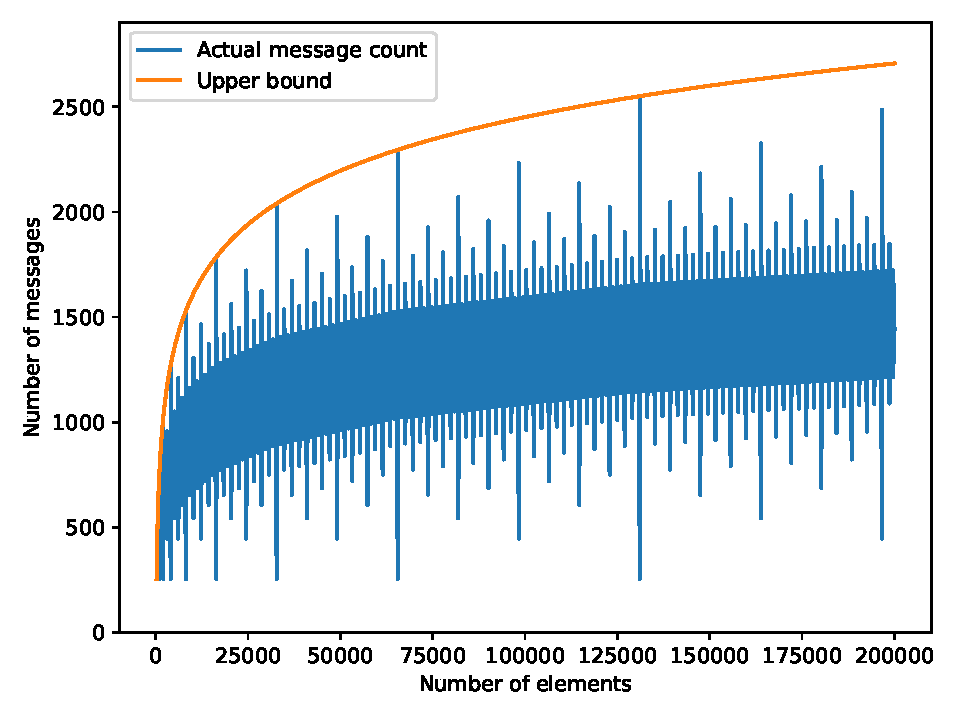
\includegraphics[width=1.0\textwidth]{figures/message_count_256.pdf}
\caption{Remaining elements assigned to the lower ranks ($n_i^\textrm{lower}$)}
\label{fig:messageCount256Lower}
\end{subfigure}
\hfill
\begin{subfigure}{0.48\textwidth}
\centering
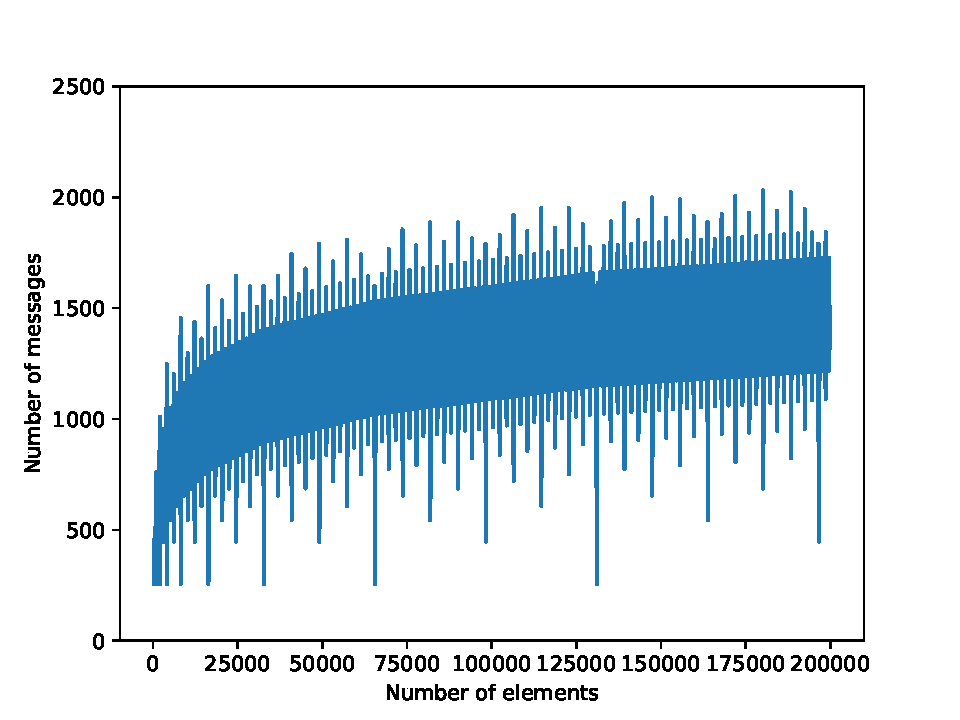
\includegraphics[width=1.0\textwidth]{figures/message_count_256_remainder_at_end.pdf}
\caption{Remaining elements assigned to the higher ranks ($n_i^\textrm{upper}$)}
\label{fig:messageCount256Upper}
\end{subfigure}
\caption{Simulated message counts for different dataset sizes on a cluster with $p=256$ \glspl{pe}.}
\label{fig:messageCount256}
\end{figure}

\Cref{fig:messageCount256} shows the number of messages depending on the dataset size for the two types of distributions introduced in \Cref{eq:lowerDistribution} and \Cref{eq:upperDistribution}.
The functions display large differences in message counts for small differences in dataset sizes, but follow a trend akin to a logarithmic function.
For $N > p$, the lower bound of the message count is $p - 1$, since all \glspl{pe} with a rank larger than $0$ must have at least one outbound subtree root in order for its elements to be included in the final result.
For the $n_i^\textrm{lower}$-distribution (\Cref{eq:lowerDistribution}), the message count attains the global minima at $N = 2^i * p$, where $i \in \mathbb{N}$.
In this case, each \gls{pe} holds an independent subtree of size $2^i$ whose root node is part of a \gls{pe}-intersecting node.
If we increase our dataset size to $N+1$, applying the $n_i^\textrm{lower}$ distribution will shift all \gls{pe}-boundaries one step in $x$-direction because of the additional element on the root \gls{pe}.
The subtree root nodes are now on different \glspl{pe} than their children, producing $i + 1$ \gls{pe}-intersecting nodes on all \glspl{pe} except the first one, as illustrated in \Cref{fig:messageCountShifting}.
Therefore, the message count for $N = 2^i * p + 1$ is 
\begin{equation}
\label{eq:messageCountI}
(p - 1) * (i + 1)
\end{equation}

Furthermore,
\begin{align*}
&N = 2^i * p + 1 \\ 
&\Leftrightarrow N - 1 = 2^i * p \\
&\Leftrightarrow \frac{N - 1}{p} = 2^i \\
&\Leftrightarrow i = \log_2 \big(\frac{N - 1}{p}\big)
\end{align*}
If we substitute $i$ in \Cref{eq:messageCountI}, we get the following closed-form upper bound on the message count for the $n_i^\textrm{lower}$ distribution:
\begin{equation}
\label{eq:upperBoundLowerDistribution}
M(N) = (p - 1) * (\log_2 \Big( \frac{N - 1}{p} \Big) + 1)
\end{equation}
\Cref{fig:messageCount256Lower} displays a plot of  \Cref{eq:upperBoundLowerDistribution} in orange color.
Under the assumption that the number of \glspl{pe} is constant, the message count $M$ therefore is in $O(\log(N))$.
Note that for the $n_i^\textrm{upper}$ distribution in \Cref{fig:messageCount256Upper}, the corresponding spikes are much less pronounced since the subtree shifting described above does not occur when adding only one element.
Because of the lower upper bound, implementations should therefore prefer the $n_i^\textrm{upper}$ distribution over the $n_i^\textrm{lower}$ distribution.

